Das folgende Kapitel zum Modbus Protokoll bezieht sich auf \cite{Modbus_Organization_AP:2012, Modbus_Organization_SL:2012}. \newline Die offizielle Definition des Modbus Protokolls von der Modbus Organization \cite{Modbus_Organization_AP:2012} lautet:
\begin{quotation}
	\emph{
		MODBUS is an application layer messaging protocol, positioned at level 7 of the OSI model, which provides client/server communication between devices connected on different types of buses or networks.}
\end{quotation}

Der Modbus Standard definiert ein Application Layer Kommunikations Protokoll, dass sich auf Schicht 7 des OSI-Modells befindet. Es bietet Client/Server Kommunikation zwischen Geräten, die auf verschiedenen Bussen oder Netzwerken angeschlossen sind.

Das Modbus Protokoll wurde 1979 von Gould-Modicon entwickelt. Aufgrund seiner offenen Art (man kann jegliche Geräte als Client anhängen) und geringer Kosten, ist das Modbus-Protokoll immer noch ein Industriestandard. Besonders oft wird das Protokoll in Mess- und Regelsystemen eingesetzt (https://www.kvm-concepts.de/wiki/m/modbus/)
https://www.kunbus.com/de/modbus 

Es gibt zwei verschiedene Einteilungen des Modbus Protokolls: 
\begin{itemize}
\item \textbf{Modbus Application Protocol:} Befindet sich auf der siebten Schicht des OSI-Modells. Dabei können die Geräte an einem Bus oder an einem Netzwerk angeschlossen werden. Genauere Information über die Ausführungsart mit dem TCP Protokoll sind später in diesem Kapitel zu finden.
\item \textbf{Modbus Serial Line Protocol:} Befindet sich auf der zweiten Schicht des OSI-Modells. Die Geräte sind hier an einem seriellen Bus angeschlossen. Dabei gibt es hier zwei Ausführungsarten, nämlich RTU und ASCII. Diese werden später ausführlicher beschrieben.
\end{itemize}

\subsection{Funktionsweise}
Modbus verwendet das Client/Server System. In einem Bussystem kann es nur einen Client geben. Es können jedoch beliebig viele Server am Bus angeschlossen werden. Der Client kann die Kommunikation mit den einzelnen Servern initialisieren. Er kann ihnen Daten senden und von ihnen Daten anfordern. Ein Server hingegen kann keine Kommunikation beginnen, sondern lediglich auf Anfrage des Clients handeln.

Jeder Server am Bus hat eine einzigartige Adresse. Die Adressen können Werte von 0 bis 255 einnehmen (siehe Tab.~\ref{tab:modbus_adressen} für die Einteilung). 
\begin{table}[h]
	\caption{Modbus Adressen Einteilung \label{tab:modbus_adressen}}
	\begin{tabularx}{\textwidth}{@{}c|c|X@{}}
		\toprule
		\textbf{Adressen} & \textbf{Bezeichnung} & \textbf{Beschreibung} \\
		\midrule
		0 & Broadcast & Hiermit sendet der Client eine Anfrage an alle Server am Bus. Diese senden keine Antwort zurück. \\
		1 - 247 & Servers & Der Client kann damit einzelne Server ansprechen. Diese senden dem Client eine Antwort zurück. \\
		248 - 255 & Reserviert & \\
		\bottomrule
	\end{tabularx}
\end{table}

Der Grundbestandteil des Modbus Protokolls ist die sogenannte \acf{pdu}. Diese besteht aus einem Function Code und den Daten. In manchen Fällen werden dem \acs{pdu} zusätzliche Felder hinzugefügt. Es kann zum Beispiel eine zusätzliche Adresse und eine Checksumme zur Fehlererkennung eingebaut werden. Das gesamte Datenpaket wird \acf{adu} genannt.
(Abb.~\ref{fig:modbus_adu_pdu}).
\begin{figure}[ht]
	\centering
	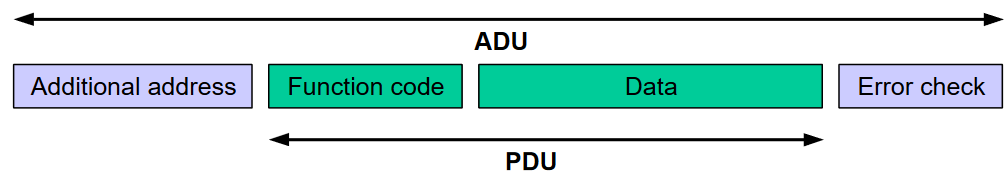
\includegraphics[width=1.0\linewidth]{Bilder/General_Modbus_Frame}
	\caption{Modbus Dataframe (Quelle: \url{https://modbus.org/docs/Modbus_Application_Protocol_V1_1b3.pdf})}
	\label{fig:modbus_adu_pdu}
\end{figure}

\begin{itemize}
	\item \textbf{Address Field:} Die Adresse des angefragten Servers bzw. mehrerer Server.
	\item \textbf{Function Code:} Dieses Feld ist ein Byte groß. Die Werte reichen von 1 bis 255, wobei 128 bis 255 für Fehlercodes vorbehalten sind. Wenn der Server eine Nachricht vom Client bekommt, zeigt ihm dieses Feld den Verwendungszweck der erhaltenen Daten an. 
	\item \textbf{Data:} In diesem Feld werden die Daten beigefügt. Außerdem sind auch zusätzliche Informationen wie die Registeradressen und die Länge der Daten enthalten. Teilweise kann dieses Feld auch Leer bleiben. In diesem Fall werden alle nötigen Informationen über die auszuführende Aktion durch den Function Code geliefert.
	\item \textbf{Error Check:} Falls bei der Übertragung einzelne Bits verändert oder verloren gehen, kann mit der Checksumme die Vollständigkeit der erhaltenen Nachricht festgestellt werden.
	Unterschied zu Function Fehlercodes: Function Fehlercodes deuten an, dass die Aktion, die der Server ausführen sollte fehlschlug. Die Checksumme prüft auf Übertragungsfehler (Behauptung: Mit fakten belegen).
\end{itemize}

Die Datenspeicherung von Modbus basiert auf sogenannten Registern. Die Register werden im Speicher des jeweiligen Geräts in einem Block zusammengefasst. Es gibt verschiedene Registertypen, die sich in der Länge der gespeicherten Daten und dem Zugriffstyp unterscheiden (siehe Tab.~\ref{tab:modbus_register_tabellen}). \newline Ein Server kann dann die Register auf den Clients mittels Anfragen auslesen oder setzen. Clients können ihre eigenen Register setzen.
\begin{table}[H]
	\caption{Modbus Register Tabellen \label{tab:modbus_register_tabellen}}
	\begin{tabularx}{\textwidth}{@{}l|c|c|X@{}}
		\toprule
		\textbf{Tabellenname} & \textbf{Datentyp} & \textbf{Zugriffstyp} & \textbf{Beschreibung} \\
		\midrule
		Input Discrete & Single bit & Read-Only & Durch \acf{io} veränderbar \\
		Coils & Single bit & Read-Write & Durch Anfragen veränderbar \\
		Input Registers & 16-bit word & Read-Only & Durch \acs{io} veränderbar \\
		Holding Registers & 16-bit word & Read-Write & Durch Anfragen veränderbar \\
		\bottomrule
	\end{tabularx}
\end{table}
(https://ipc2u.de/artikel/wissenswertes/modbus-rtu-einfach-gemacht-mit-detaillierten-beschreibungen-und-beispielen/)

Jeder dieser Blöcke hat einen separaten Bereich im Speicher (Siehe Abb.~\ref{fig:modbus_register_many_blocks}):
\begin{figure}[H]
	\centering
	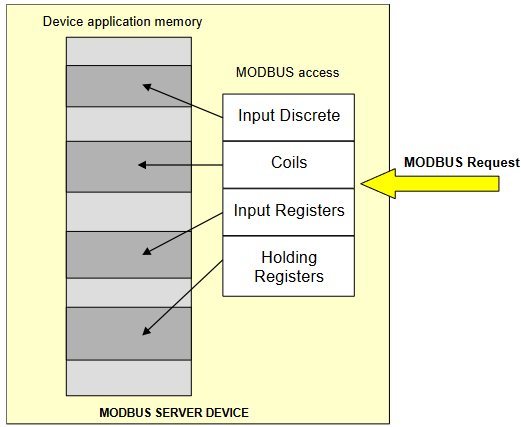
\includegraphics[width=0.4\linewidth]{Bilder/Modbus_Data_Model_with_separate_block}
	\caption{Modbus Daten in separaten Blöcken (Quelle: \url{https://modbus.org/docs/Modbus_Application_Protocol_V1_1b3.pdf})}
	\label{fig:modbus_register_many_blocks}
\end{figure}

Oder die Blöcke sind zusammengeschaltet und können durch unterschiedliche Eingaben erreicht werden (Abb.~\ref{fig:modbus_register_one_block}).
\begin{figure}[H]
	\centering
	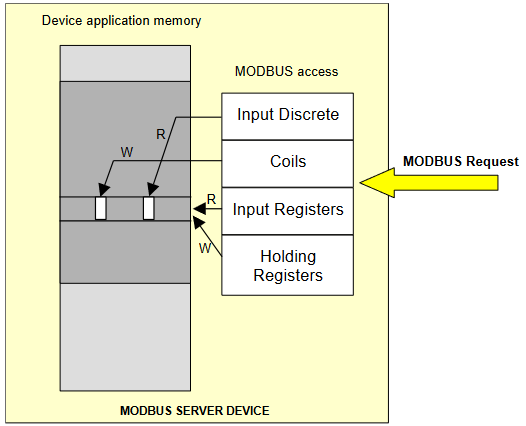
\includegraphics[width=0.4\linewidth]{Bilder/Modbus_Data_Model_with_one_block}
	\caption{Modbus Daten in einem Block (Quelle: \url{https://modbus.org/docs/Modbus_Application_Protocol_V1_1b3.pdf})}
	\label{fig:modbus_register_one_block}
\end{figure}

\subsection{Übertragungsarten}
Es gibt verschiedene Übertragungsarten. Für die serielle Schnittstelle, gibt es \acf{rtu} und \acf{ascii}. Auf einem seriellen Bus, müssen alle Geräte die selbe Übertragungsart verwenden. Der \acs{rtu} Modus ist dabei der Standard, den alle Modbus Geräte implementieren müssen. \acs{ascii} kann optional verwendet werden. \newline Es gibt auch noch \acs{tcp} und Modbus Plus. Diese beiden Übertragungsarten sind für diese Diplomarbeit nicht relevant. Daher wird auf eine genauere Beschreibung verzichtet.

\paragraph{\acs{rtu} Modus}
Bei dem \acs{rtu} Modus werden 8-bit Datenbytes nacheinander gesendet. In den meisten Programmen werden diese 8-Datenbits von 2 hexadezimalen Zahlen dargestellt. Die Übertragung muss dabei ununterbrochen stattfinden. Im Vergleich zu \acs{ascii} ist bei \acs{rtu} der Datendurchsatz höher. 

Die Nachricht besteht aus 11 bits und wird folgendermaßen aufgeteilt:
\begin{itemize}
	\item \textbf{1 Startbit:} Signalisiert dem Empfänger, dass eine Nachricht folgt
	\item \textbf{8 Datenbits:} Die eigentlichen Daten
	\item \textbf{1 Paritätsbit:} Stellt fest, ob alle Datenbits richtig empfangen wurden. Es zeigt an, ob die Summe der empfangene Datenbits gerade (even) oder ungerade (odd) ist. Ob die Summe gerade ist oder ungerade wird dann mit dem Paritätsbit verglichen.   (https://www.ibm.com/docs/de/aix/7.3?topic=parameters-parity-bits) Es können 3 verschiedene Modi eingestellt werden: even, odd oder no parity.
	\item \textbf{1/2 Stopbits:} Signalisiert dem Empfänger, dass die Nachricht endet. Wenn no parity eingestellt wurde, gibt es 2 Stopbits, dafür aber kein Paritätsbit.
\end{itemize}

Nach jeder Nachricht wird 3.5 Zeichen gewartet, bis die nächste Nachricht versendet wird. Dadurch
erkennt das Protokoll genau, wann die nächste Nachricht anfängt. 
Bild von Seite

Benutzt CRC: ganz kurze erklärung

Diese Übertragungsart wird in den Geräten bei Bösch verwendet. Daher verwendet auch die RLT Anzeige den \acs{rtu} Modus.

\paragraph{\acs{ascii} Modus}
Ähnlich wie RTU aber doch anders: 2 ASCII characters versendet.
Zum Einleiten einer neuen Nachricht wird hier ein ":" Zeichen gesendet. Dieses ist für diesen Zweck reserviert.
(https://www.simplymodbus.ca/ASCII.htm)

Die Nachricht besteht aus 10 bits und wird folgendermaßen aufgeteilt:
\begin{itemize}
	\item \textbf{1 Startbit}
	\item \textbf{7 Datenbits}
	\item \textbf{1 Paritätsbit}
	\item \textbf{1/2 Stopbits}
\end{itemize}

Benutzt LRC: ganz kurze erklärung

\subsection{Serielle Kommunikation (bei RTU/RS485)}


%\subsection{Vor- und Nachteile}